%!TEX encoding = UTF-8 Unicode
%- Como pensam testar a solucao e validar a vossa idea, que processo vao
%  utilizar durante o desenvolvimento para facilitar a rrealizacao de testes e a
%  recolha de resultados.
%- Pretendo usar um prototipo: que equipamentos/linguagens de programacao a usar
\chapter{Evaluation Methodology}
\label{sec:Evaluation}
The evaluation of the proposed architecture will be performed both in qualitatively and quantitatively manner. The former will be assessing by evaluating if the objectives defined in Section \ref{subsec:Objectives} were effectively accomplished. Meanwhile, the latter will be responsible for the evaluation of performance metrics in terms of computational overheads in the orchestrator(s), bandwidth minimization, energy consumption reduction, cost shrinkage to the infrastructure service providers, and the QoS offered to the end users. After the implementation of the extensions that are in sight to be implemented in the simulator (refer to Section \ref{sec:Architecture}), it will be possible to evaluate the system by simulating a similar controlled environment as depicted in Figure \ref{fog_setup}. The connections were already discussed in Section \ref{sec:fog_architecture}, specifically in Figure \ref{fog_architecture}.\\
\noindent\tab The qualitative evaluation will be performed through the following appreciations:
\begin{itemize}[noitemsep]
	\item Verify if the simulator is correctly able to support horizontal communication;% rather than parent-child only;
	\item Check if the implemented optimization algorithms actually converge and give a proper solution;
	\item Test mobile environments similar to what is depicted in Figure \ref{fog_setup};
	\item Verify if the optimization algorithms still converge in mobile environments.
\end{itemize}
\noindent\tab Regarding quantitative evaluation, it will be given special attention to the following metrics:
\begin{itemize}[noitemsep]
	\item Analise both complexity and execution time of each optimization algorithm;
	\item Measure the QoS offered to applications and if its time boundaries are met with each algorithm;
	\item Compare those values with the ones offered by the current version of iFogSim; %in a static environment;
	\item Measure values of bandwidth usage, energy consumption, and cost for infrastructure service providers achieved in both static and dynamic environments with each algorithm;
	\item Compare the obtained results for the static environment with the values achieved by iFogSim.
\end{itemize}
\begin{figure}[h]
	\centering
	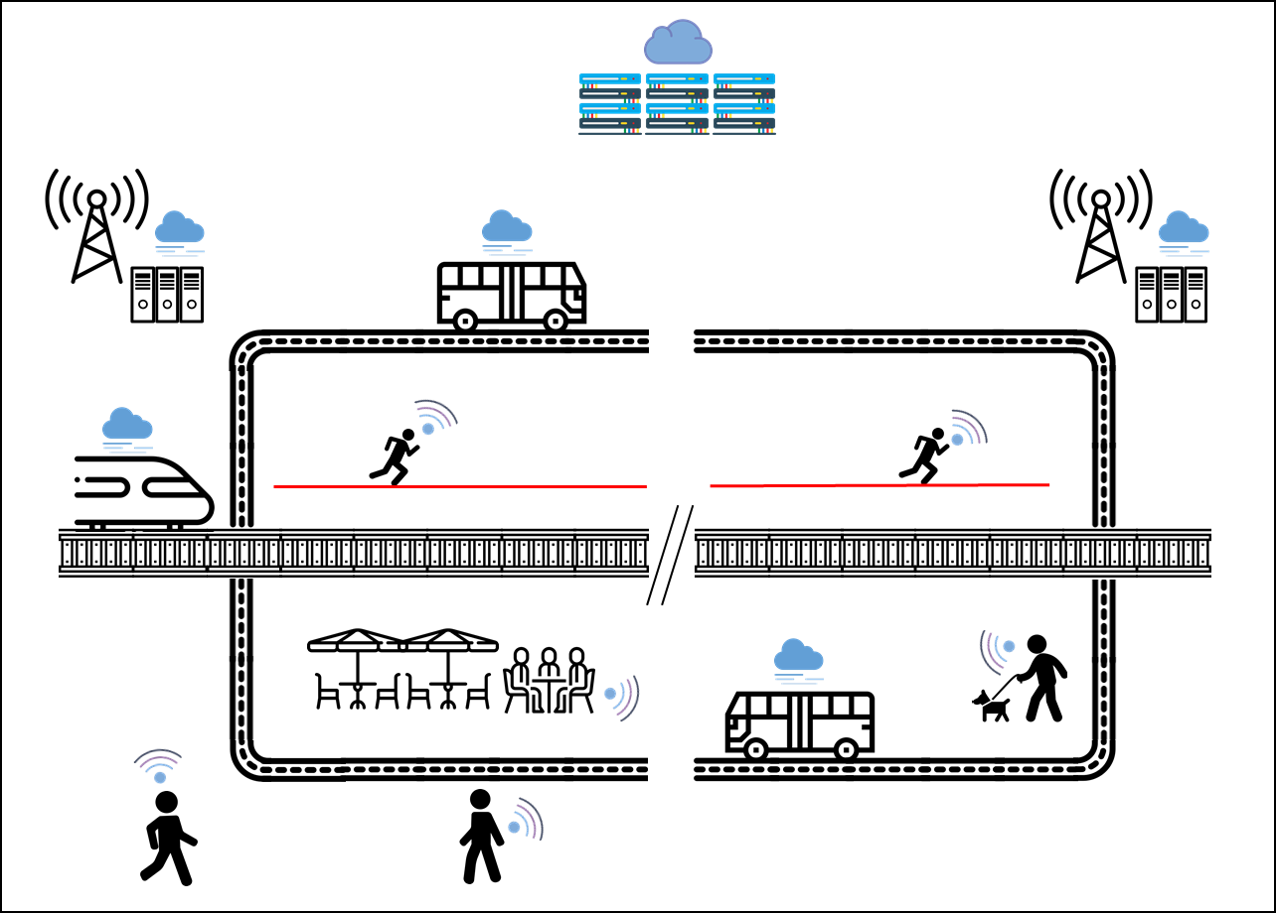
\includegraphics[width=.45\textwidth]{images/evaluation/evaluation.png}
	\caption{Example of setup to evaluate the system and its performance.}
	\label{fog_setup}
\end{figure}